\begin{frame}[fragile]
\frametitle{Fast and Loose Reasoning}
\begin{fact}Non-totality is a consequence of any turing-complete system\end{fact}
\end{frame}

\begin{frame}[fragile]
\frametitle{Fast and Loose Reasoning}
\begin{itemize}
  \item This means that any turing-complete system will permit \emph{escape hatches for partiality}.
  \item Each turing-complete system has different, specialised mechanisms that permit partiality.
  \item These escape hatches undermine the value of our assertions \ldots but let's not throw away everything.
\end{itemize}
\end{frame}

\begin{frame}[fragile]
\frametitle{Fast and Loose Reasoning}
\begin{block}{Scala has a \sout{few} lot of escape hatches}
\begin{itemize}
  \item \lstinline{null}
  \item exceptions
  \item Type-casing (\lstinline{isInstanceOf})
  \item Type-casting (\lstinline{asInstanceOf})
  \item Side-effects
  \item \lstinline{equals}/\lstinline{toString}/\lstinline{hashCode}
  \item \lstinline{notify}/\lstinline{wait}
  \item \lstinline{classOf}/\lstinline{.getClass}
  \item General recursion
\end{itemize}
\end{block}
\end{frame}

\begin{frame}[fragile]
\frametitle{Fast and Loose Reasoning}
\framesubtitle{\lstinline{null} escape hatch}
\begin{lstlisting}[style=scala]
def `irrelevant`[A](x: List[A]): List[A] = 
  null
\end{lstlisting}
\begin{theorem}Every \lstinline{A} element in the result list appears in the input list\end{theorem}
Well, not if you don't even have a list.
\end{frame}

\begin{frame}[fragile]
\frametitle{Fast and Loose Reasoning}
\framesubtitle{\lstinline{type-casing} escape hatch}
\begin{lstlisting}[style=scala]
def `irrelevant`[A](x: A): Boolean = 
  x.isInstanceOf[Int] ||
  x match {
    case (s: String) => s.length < 10
  }
\end{lstlisting}
\begin{theorem}This function ignores its argument and consistently returns either \lstinline{true} or \lstinline{false}\end{theorem}
Type-casing\footnote{case-analysis on type} breaks parametricity and so undermines our theorems.
\end{frame}

\begin{frame}[fragile]
\frametitle{Fast and Loose Reasoning}
\framesubtitle{\lstinline{type-casting} escape hatch}
\begin{lstlisting}[style=scala]
def `irrelevant`[A](x: List[A]): List[A] = 
  "abc".asInstanceOf[A] :: x  
\end{lstlisting}
\begin{theorem}Every \lstinline{A} element in the result list appears in the input list\end{theorem}
\end{frame}

\begin{frame}[fragile]
\frametitle{Fast and Loose Reasoning}
\framesubtitle{\lstinline{side-effect} escape hatch}
\begin{lstlisting}[style=scala]
def `irrelevant`[A](x: A): A = {
    println("hi")
    x
  }
\end{lstlisting}
\begin{theorem}This function only ever does one thing \textemdash return its argument \end{theorem}
\end{frame}

\begin{frame}[fragile]
\frametitle{Fast and Loose Reasoning}
\framesubtitle{\lstinline{toString} escape hatch}
\begin{lstlisting}[style=scala]
def `irrelevant`[A](x: A): Int =
  x.toString.length
\end{lstlisting}
\begin{theorem}This function ignores its argument to return one of {${2^{32}}$} values. \end{theorem}
\end{frame}

\begin{frame}[fragile]
\frametitle{Fast and Loose Reasoning}
\framesubtitle{where to place our trust?}
\begin{lstlisting}[style=scala]
def reverse[A, B](x: List[A]): List[B] = 
  x.foldLeft[List[B]](Nil)((b, a) =>
    a.`asInstanceOf`[B] :: b)
\end{lstlisting}
\begin{theorem}This function \textbf{always} returns \lstinline{Nil} and so cannot possibly reverse the list\end{theorem}
\end{frame}

\begin{frame}[fragile]
\frametitle{Fast and Loose Reasoning}
\begin{itemize}
  \item Scala sure does have a lot of escape hatches!
  \item to what extent do they pervade our reasoning abilities?
  \item let us reframe the question
  \item if we abandon all these escape hatches, to what extent is the programming environment disabled?
\end{itemize}
\end{frame}

\begin{frame}[fragile]
\frametitle{Fast and Loose Reasoning}
\begin{itemize}
  \item Haskell disables side-effects, type-casing and type-casting, \emph{obtaining a total, relative advantage}.
  \item Agda goes further by disabling non-termination, again to its advantage.
  \item so what about Scala?
  \item can we use a reliable subset without too much penalty?
\end{itemize}
\end{frame}

\begin{frame}[fragile]
\frametitle{Fast and Loose Reasoning}
\frametitle{Safe Scala subset}
\begin{center}
Yes.
\end{center}
\begin{center}
And we do.
\end{center}
\end{frame}

\begin{frame}[fragile]
\frametitle{Fast and Loose Reasoning}
\begin{block}{Safe Scala subset}
\begin{itemize}
  \item \sout{\lstinline{null}}
  \item \sout{exceptions}
  \item \sout{Type-casing (\lstinline{isInstanceOf})}
  \item \sout{Type-casting (\lstinline{asInstanceOf})}
  \item \sout{Side-effects}
  \item \sout{\lstinline{equals}/\lstinline{toString}/\lstinline{hashCode}}
  \item \sout{\lstinline{notify}/\lstinline{wait}}
  \item \sout{\lstinline{classOf}/\lstinline{.getClass}}
  \item General recursion
\end{itemize}
\end{block}
\end{frame}

\begin{frame}[fragile]
\frametitle{Fast and Loose Reasoning}
\begin{block}{Safe Scala subset}
\begin{itemize}
  \item<1> We have now \textbf{improved} our reasoning abilities, but at what cost?
  \item<2> It turns out that eliminating these escape hatches results in a \textbf{significant language improvement} with minimal, orthogonal, easily-managed penalties.
  \item<3> In other words, we can assume the language subset absent these attributes and by doing so, achieve a large net benefit.
\end{itemize}
\end{block}
\end{frame}

\begin{frame}[fragile]
\frametitle{Fast and Loose Reasoning}
\begin{itemize}
  \item<1> Fast and loose reasoning justifies reasoning as if we were in a total language
  \item<2> But it does not justify letting go of any possible reasoning ability
\end{itemize}
\end{frame}

\begin{frame}[fragile]
\frametitle{Fast and Loose Reasoning}
\framesubtitle{The propose compromise of mistrust and pessimism}
\begin{itemize}
  \item<1> If we are uncomfortable with, or defeatist toward using the type system for reasoning about code \ldots
  \item<2> \ldots then is it any wonder that we see scrambling for unreliable and inaccurate comprehension mechanisms, such as stressing the importance of identifier names?
\end{itemize}
\end{frame}

\begin{frame}[fragile]
\frametitle{Fast and Loose Reasoning}
\framesubtitle{It works}
\begin{itemize}
  \item<1> There are plenty of open-source projects, in Scala, even Java and C\#, where fast and loose reasoning applies
  \item<2> Project contributors rarely step on each others' (or their own) toes precisely because of this optimistic approach
  \item<3> and when they do, the consequences are minimal
\end{itemize}
\end{frame}

\begin{frame}[fragile]
\frametitle{Fast and Loose Reasoning}
\framesubtitle{It works}
\begin{center}
Parametricity is principled and it works
\end{center}
\begin{center}
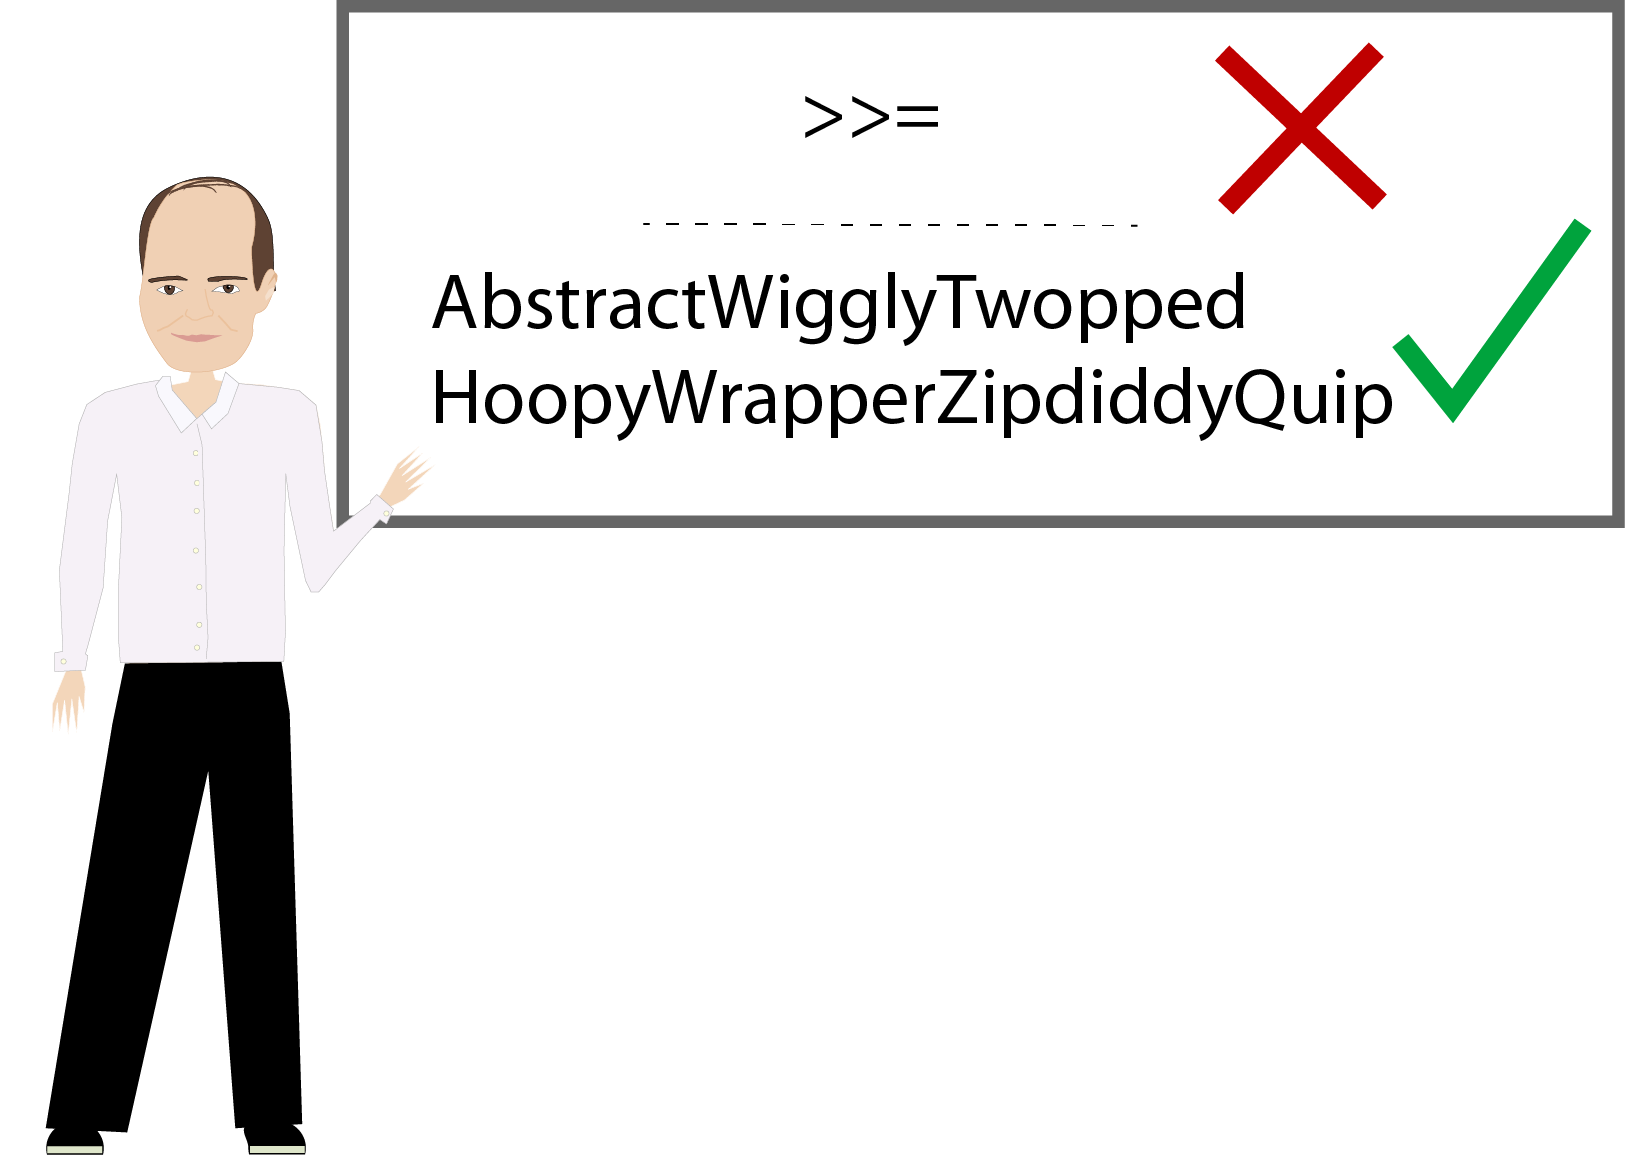
\includegraphics[height=3.8cm]{image/AbstractWigglyTwoppedHoopyWrapperZipdiddyQuip.png}
\end{center}
\begin{center}
If you do not exploit it, I will judge you
\end{center}
\end{frame}
